\begin{figure*}[t]
\centering
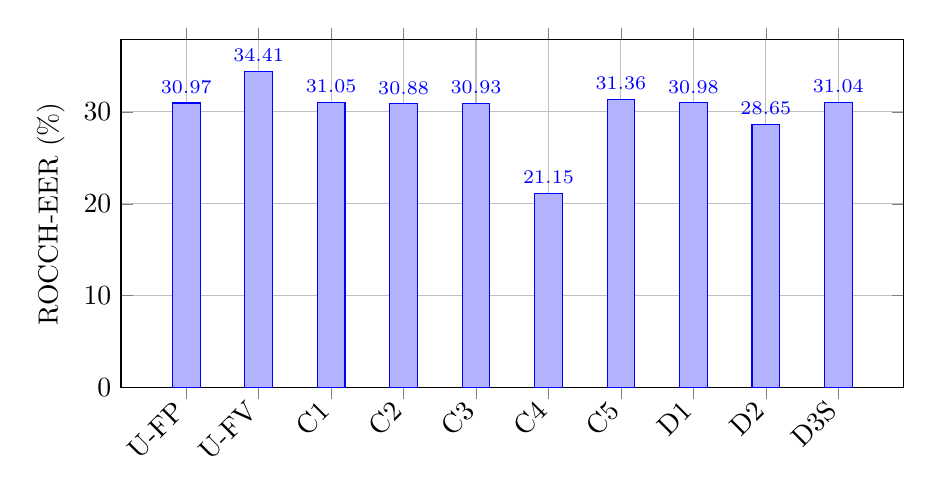
\begin{tikzpicture}
\begin{axis}[ybar, width=0.95\textwidth, height=6cm, ymin=0, ylabel={ROCCH-EER (\%)}, symbolic x coords={U-FP,U-FV,C1,C2,C3,C4,C5,D1,D2,D3S}, xtick=data, x tick label style={rotate=45,anchor=east}, nodes near coords, nodes near coords style={font=\scriptsize}, grid=major]
\addplot coordinates {(U-FP,30.969136) (U-FV,34.406793) (C1,31.053879) (C2,30.876043) (C3,30.928887) (C4,21.146749) (C5,31.362543) (D1,30.983505) (D2,28.645278) (D3S,31.040809)};
\end{axis}
\end{tikzpicture}
\caption{Clean-condition discrimination on the locked V1 final trials. Lower is better.}
\label{fig:v1-clean-eer}
\end{figure*}
